\chapter{Réalisation}
	
\section{Introduction}
Ce chapitre constitue le dernier volet de ce rapport, il traite la phase qui a pour objectif l’implantation de notre application. Nous commençons par la description de l’environnement logiciel utilisé pour développer notre solution et les différentes fonctionnalités réalisées. Ensuite nous terminons par exposer l'écart entre la réalisation réelle et les taches planifiées au niveau du premier chapitre.
\section{Environnement de développement}
Afin de construire notre application, nous avons utilisé un ensemble de Framework, environnement de développement et outils
de conception, c'est ce que nous présenterons dans cette section.\\
L’environnement logiciel employé est le suivant :
\begin{itemize}
\item \textbf{WAMP}: Nous avons déployé nos intergiciels sous WAMP, vu qu’il propose les dernières mises à jour du langage PHP. En plus, il intègre plusieurs bibliothèques open source.
\item \textbf{Postman} : Nous avons testé nos services web grâce à l’outil Postman qui nous a permis de tester les requêtes HTTP et les interpréter en dehors du contexte métier.
\item \textbf{PHPStorm}: PhpStorm est un éditeur pour PHP, HTML, CSS et JavaScript, produit par JetBrains.
Il est compatible avec Git ce qui a facilité la procédure de gestion de versions au cours du développement de notre application.
Il est payant, sauf dans certains cas comme pour les étudiants ou les projets open source.
\end{itemize}

\section{Choix technologiques et langages utilisés}
Dans cette section, nous allons citer nos choix technologiques et les langages que nous avons utilisés pour mener à bien ce projet.
\subsection{WEB API RESTful}
Afin d’assurer l’interaction entre le back-end et le front-end de l'application, nous avons implémenté des services web PHP de type REST.
Les réponses sont sous format JSON puisque il est plus légère et facile à manipuler.
\subsection{Symfony 3.4}
Symfony est un framework MVC libre écrit en PHP 5. Il fournit des fonctionnalités qui permettent de faciliter et d’accélérer le développement d'un site web. 
\section{Planning réel du projet}
Nous présentons au cours de cette section, les durées réelles des tâches que nous avons
planifiées au niveau du premier chapitre.
Dû aux problèmes imprévus qui ont apparût lors de la réalisation de notre projet, nous
n’avons pas estimer les durées exactes de nos tâches.  \ref{fig6}.
\begin{figure} [H]
    \centering
         \begin{center}
             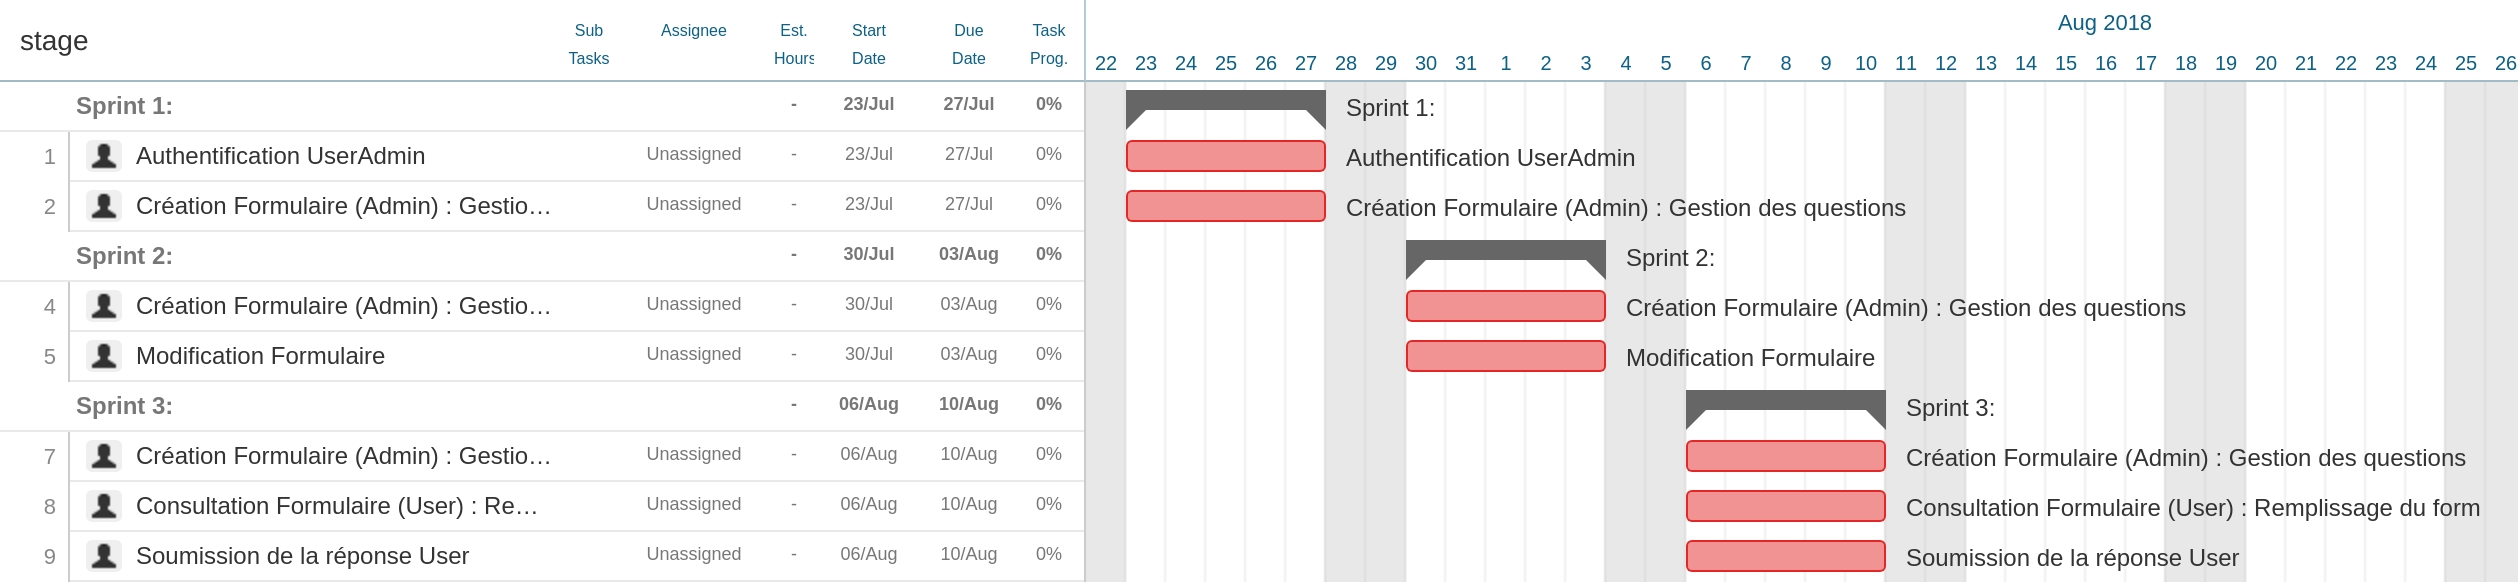
\includegraphics [width=16cm,height=8cm] {img/GANTTdiag.jpg}
            \caption{Réalisation en temps réel }
            \label{fig6}
        \end{center}
    \end{figure}
    
\section{Test des services web}
Les tests sont effectués grâce à l'outil Postman tout en introduisant l'url correspondant à l'API créee et la méthode HTTP utilisée avec un format de retour des données JSON.\\
La figure \ref{login} présente un succès d'authentification d'un administrateur.
\begin{figure} [H]
    \centering
         \begin{center}
             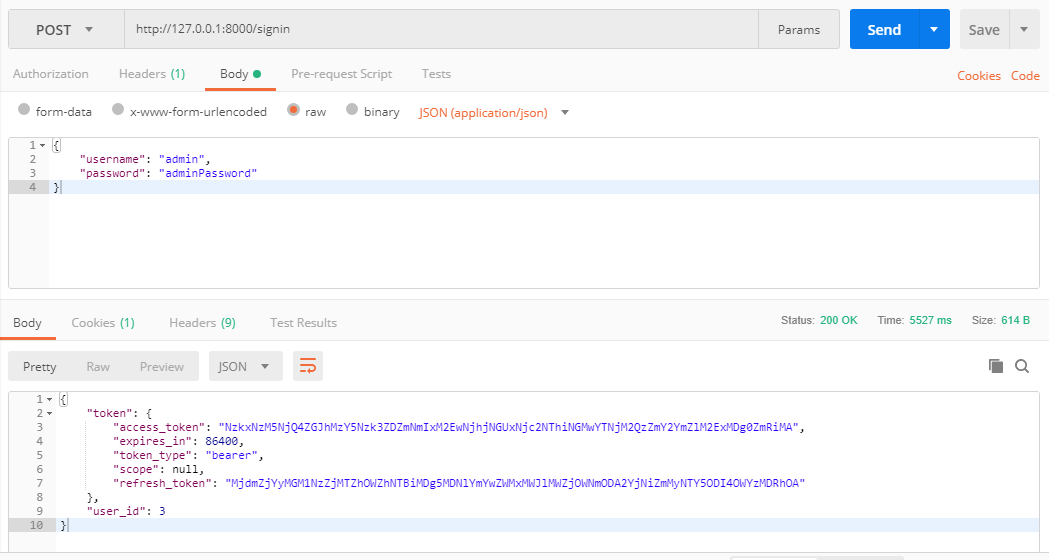
\includegraphics [width=16cm,height=9cm] {SprintImage/loginSuccess.PNG}
            \caption{Web Service "Signin"}
            \label{login}
        \end{center}
    \end{figure}
    
    La figure \ref{SerWeb1} illustre le service web permettant la soumission d'un formulaire, la figure \ref{SerWeb2} son affichage et la modification avec la figure \ref{SerWeb3}.

    \begin{figure} [H]
    \centering
         \begin{center}
             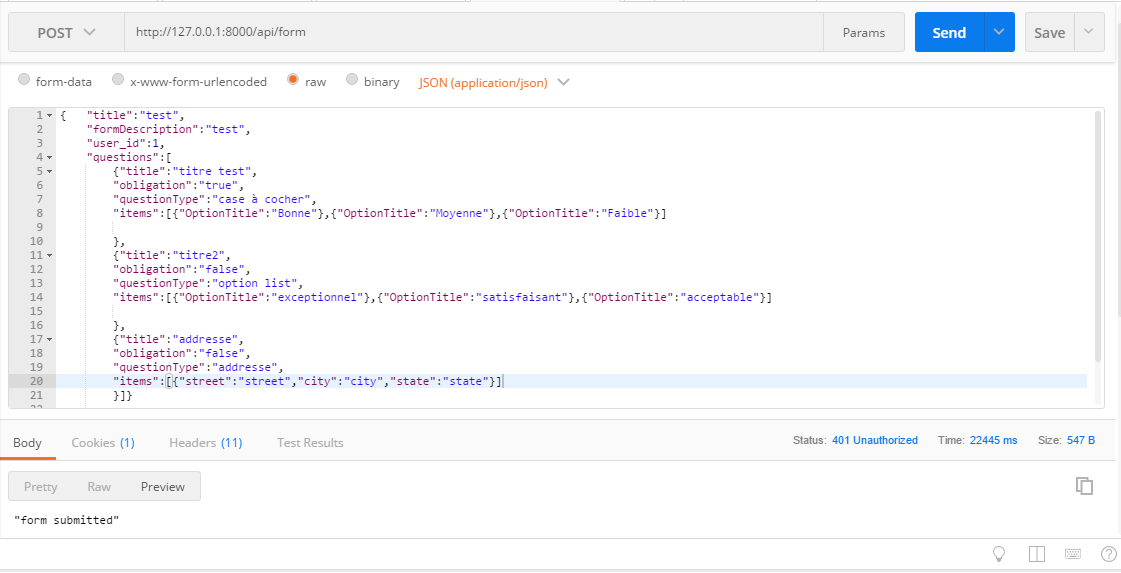
\includegraphics [width=16cm,height=9cm] {SprintImage/FormSubmitted.png}
            \caption{Web Service " Soumettre un formulaire"}
            \label{SerWeb1}
        \end{center}
    \end{figure}
    
    \begin{figure} [H]
    \centering
         \begin{center}
             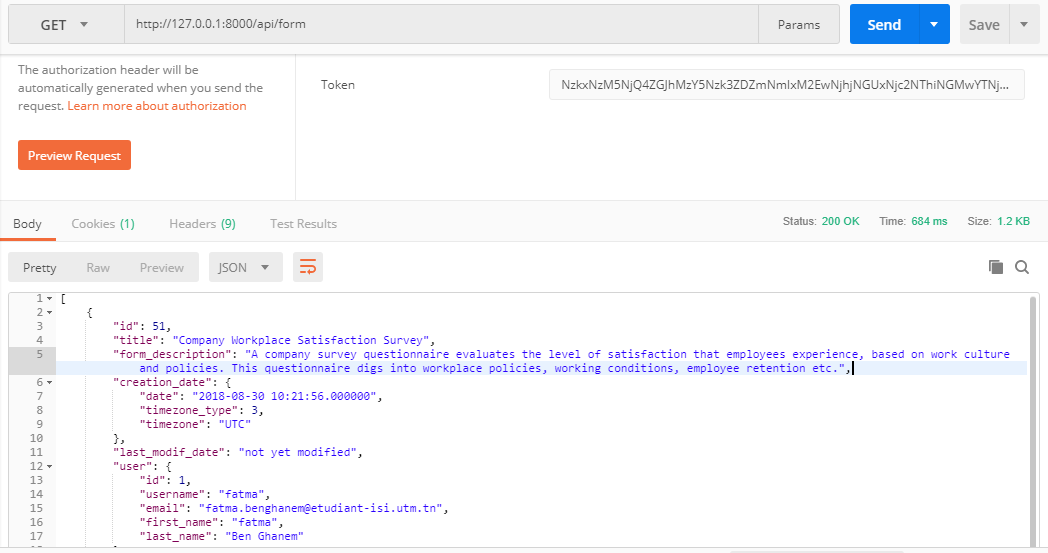
\includegraphics [width=16cm,height=9cm] {SprintImage/GetForms.PNG}
            \caption{Web service "affichage des formulaires"}
            \label{SerWeb2}
        \end{center}
    \end{figure}
    
    \begin{figure} [H]
    \centering
         \begin{center}
             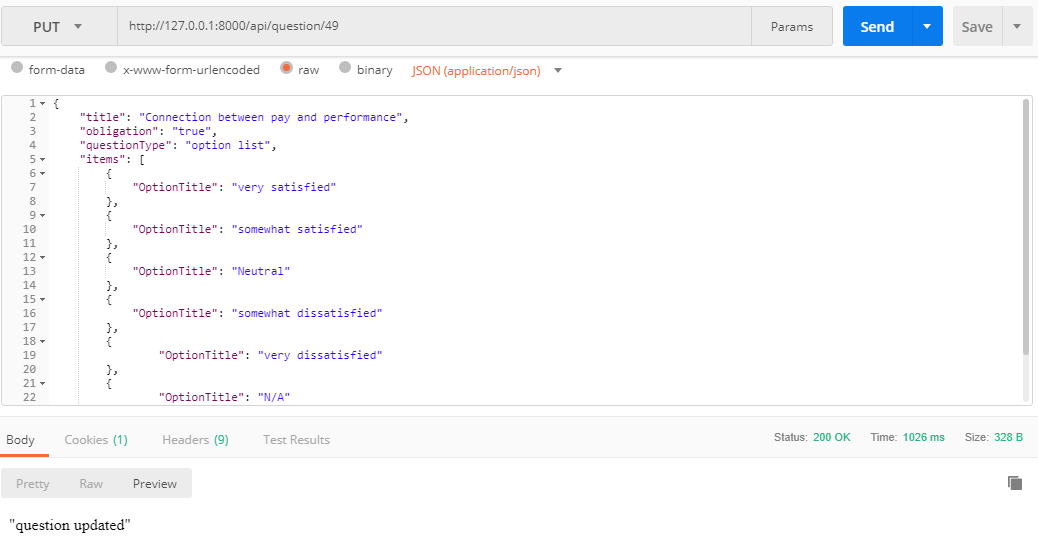
\includegraphics [width=16cm,height=9cm] {SprintImage/PutQuestion.PNG}
            \caption{Web service "modification formulaire"}
            \label{SerWeb3}
        \end{center}
    \end{figure}
    \newpage
     La figure \ref{fig5} illustre la soumission d'une réponse.
\begin{figure} [H]
    \centering
         \begin{center}
             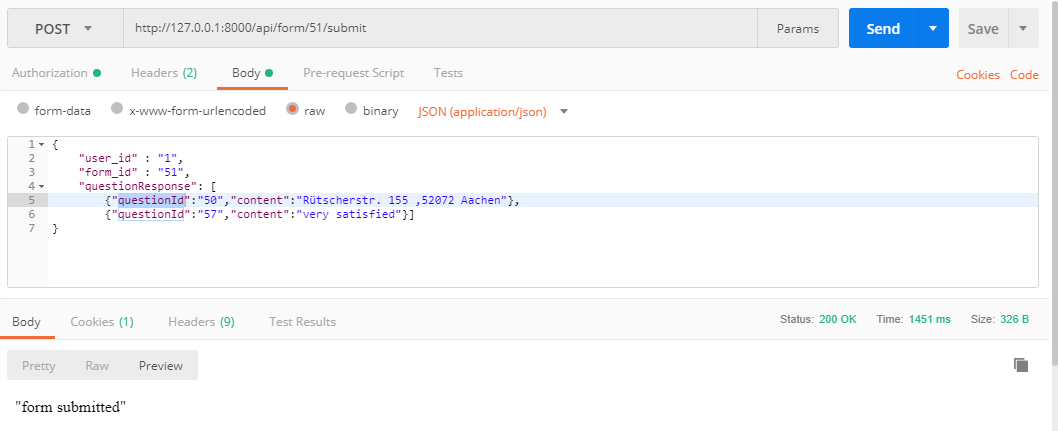
\includegraphics [width=16cm,height=7cm] {SprintImage/submitForm.PNG}
            \caption{Soumettre la réponse }
            \label{fig5}
        \end{center}
    \end{figure}

\section{Conclusion}
Nous avons réalisé au niveau de ce dernier chapitre, le choix de l’ensemble des composants logiciels combinés aux variantes techniques adoptées, ainsi que quelques artefacts de la gestion de projet.